\documentclass[11pt, a4paper, oneside]{article} 
% use "amsart" instead of "article" for AMSLaTeX format
%\usepackage{mydefs,mythm}
\usepackage[textsize=footnotesize,textwidth=3cm]{todonotes}
% \geometry{landscape} % Activate for rotated page geometry
% \usepackage[parfill]{parskip} % Activate to begin paragraphs with an empty line rather than an indent
\setlength{\parindent}{0pt}
\addtolength{\parskip}{7pt}

\newcommand{\Lam}{\Lambda}
\newcommand{\Lamc}{{\bar{\Lambda}}}
\usepackage{amsthm}
\newtheorem{thm}{Theorem}
\newtheorem{theorem}[thm]{Theorem}
\newtheorem{conj}[thm]{Conjecture}
\newtheorem{conjecture}[thm]{Conjecture}
\newtheorem{cor}[thm]{Corollary}
\newtheorem{corollary}[thm]{Corollary}
\newtheorem{lem}[thm]{Lemma}
\newtheorem{lemma}[thm]{Lemma}
\newtheorem{prop}[thm]{Proposition}
\newtheorem{proposition}[thm]{Proposition}

\newtheorem{ax}{Axiom}
\newtheorem{axiom}{Axiom}
\newtheorem{claim}{Claim}
\theoremstyle{definition}
\newtheorem{defn}{Definition}
\newtheorem{definition}{Definition}
\newtheorem{ex}{Example}
\newtheorem{example}{Example}
\theoremstyle{remark}
\newtheorem{notation}{Notation}
\newtheorem{remark}{Remark}
\newtheorem{rem}{Remark}

\PassOptionsToPackage{override}{xcolor} % Beamer option
\usepackage[utf8]{inputenc}
\usepackage{hyperref}
\usepackage{subfig}
\usepackage{amsmath} 
\usepackage{amssymb}
\usepackage{amsfonts,amssymb}
\usepackage{dsfont}
\usepackage[mathscr]{euscript}
\usepackage{enumerate,xspace,threeparttable}
\usepackage{graphicx}
\usepackage{verbatim}
\usepackage{algorithmic}
\usepackage{listings}
\usepackage{wrapfig}
\usepackage{translator}

\providecommand{\ie}{i.e.\ }
\providecommand{\qr}{\eqref}
\renewcommand{\d}{\,d}
\providecommand{\dd}[2]{\dfrac{d#1}{d#2}}
\providecommand{\qtext}[1]{\quad\text{#1 }\quad}

\providecommand{\RR}{\mathbb{R}}
\providecommand{\CC}{\mathbb{C}}
\providecommand{\TT}{\mathbb{T}}
\providecommand{\ZZ}{\mathbb{Z}}
\providecommand{\QQ}{\mathbb{Q}}
\providecommand{\NN}{\mathbb{N}}
\providecommand{\VV}{\mathbb{V}}
\providecommand{\PP}{\mathsf{P}}
\providecommand{\EE}{\mathsf{E}}
\providecommand{\BB}{\mathbb{B}}
\renewcommand{\SS}{\mathbb{S}}

\providecommand{\CF}{\mathscr{F}}
\providecommand{\CB}{\mathscr{B}}
\providecommand{\CA}{\mathscr{A}}
\providecommand{\CR}{\mathscr{R}}
\providecommand{\CH}{\mathscr{H}}
\providecommand{\CM}{\mathscr{M}}
\providecommand{\CT}{\mathscr{T}}

\providecommand{\mfrak}{\mathfrak}
\providecommand{\mscr}{\mathscr}
\providecommand{\mc}{\mathcal}
\providecommand{\mb}{\mathbf}
\providecommand{\bs}{\boldsymbol}
\providecommand{\mbb}{\mathbb}
\providecommand{\ms}{\mathsf}
\providecommand{\vv}[2]{\ensuremath{\overrightarrow{#1#2}}} % vector
\providecommand{\opn}{\operatorname}
\providecommand{\ol}{\overline}
\def\ii#1{^{(#1)}}
\providecommand{\E}{\mathsf{E}}
\renewcommand{\P}{\mathsf{P}}
\renewcommand{\Pr}[1]{\P\left(#1\right)}
\providecommand{\Ex}[1]{\E(#1)}

\providecommand{\Var}{\opn{Var}}
\providecommand{\var}{\opn{var}} 
\providecommand{\Cov}{\opn{Cov}}
\providecommand{\sign}{\opn{sign}}
\providecommand{\diag}{\opn{diag}}

\providecommand{\msf}{\mathsf}
\providecommand{\ett}{\mathsf{1}}

\providecommand{\Ordo}[1]{{O(#1)}} 
\providecommand{\ordo}[1]{{o(#1)}} 
\providecommand{\OrdoOmega}[1]{{\varOmega(#1)}} 
\providecommand{\OrdoTheta}[1]{\ensuremath{\Theta(#1)}} 
\providecommand{\ordoomega}[1]{\ensuremath{\omega(#1)}}

\providecommand{\e}{\epsilon}
\providecommand{\tl}{\tilde}
\providecommand{\g}{\gamma}
\providecommand{\w}{\omega}
\providecommand{\C}{C}
\providecommand{\scp}[2]{\ensuremath{\left\langle#1,#2\right\rangle}}

\providecommand{\bmat}[1]{\begin{bmatrix} #1 \end{bmatrix}}
\providecommand{\T}{^{\!\mathrm{T}}}
\providecommand{\ds}{\displaystyle}

\renewcommand{\L}{\mathscr{L}}

\def\Ex#1{\EE\left[#1\right]}

\def\dom{\opn{dom}}

\def\X{\mscr X}
\def\T{\opn{\msf{T}}}


\def\ilim{\varinjlim}
\def\plim{\varprojlim}
\def\lover#1{\overset{#1}{\longleftarrow}}
\def\rover#1{\overset{#1}{\longrightarrow}} 
\def\npair#1#2{\left\langle\, #1\mid #2\,\right\rangle}
\def\F{\mscr F}

\def\scp#1#2{\left\langle #1 , #2 \right\rangle}

\def\e{\varepsilon}

\title{Existence for an eigenfunction for the sub-critical phase of the Dyson
  Ising model\langle{}\rangle}

\author{Anders Johansson, Anders \"Oberg, Mark Pollicott, \\ and Evgeny Verbitskiy}
\date{}
\begin{document}
\maketitle


\section{Introduction}\noindent


\def\gibb{\dot\ltimes} \def\gibbs{\ltimes}

\subsection{The random cluster model and potentials}

We consider measures $\alpha \in \mscr M(X)$ on configuration spaces $X = A^S$,
where $A$ is a finite set (the ``alphabet'') and $S$ (the ``sites'') is a
countable and usually infinite. A \emph{potential} $\phi(x)$ on $X$ is a limit
$\phi(x) = \lim_{n\to\infty}\phi_n(x)$ of functions such that the difference
$\phi(x)-\phi(y)$ is finite and well defined for any pair of configurations $x$
and $y$ that coincide outside any finite set $\Lambda\subset S$. Given a
probability measure $\alpha$ on $X$ and a potential $\phi$ on $X$, we denote by
\[
  e^{s\phi(x)} \gibbs \d\alpha(x)
\]
the family of \emph{Gibbs measure}, i.e.\ the weak limits $\Lambda\nearrow S$ of
\[
  p_\Lambda(x\vert_\Lambda\mid x\vert_{\Lambda^c}) = \frac {e^{s\phi(x)}\alpha(x\vert_{\Lambda}\mid x\vert_{\Lambda^c})} {Z_\Lambda(x\vert_{\Lambda^c})}
\]

Examples of unique Gibbs measures are Bernoulli measures.

\subsection{The one-dimensional Random cluster model and the Ising-Dyson model}

For a finite graph, let $\w(G)$ denote the number of connected components
(``clusters'') in the graph $G$. For simple graphs $G\subset \binom V2$ on an
countably infinite set $V$ of vertices, we consider the number of clusters
$\w(G)$ as a \emph{potential}. This means that the difference
$\Delta\w(G,F) = \w(G)-\w(F)$ is defined for any two graphs $F$ and $G$ that
coincide outside a \emph{finite} subset $\Lambda\subset \binom V2$.

A random graph $G\sim\alpha$ on a set of vertices $V$ is a probability
distribution $\alpha$ on the set $\{0,1\}^{\binom V2}$. The random cluster
models $\mscr R(V,p)$, we consider are specified by a set of vertices $V$ and a
weight function $p$, $ij\mapsto p(ij)\in[0,1]$, defined on the set of pairs
$ij\in \binom V2$. The model $\mscr R(V,p)$ is a Gibbs distribution on random
graphs, i.e.\ configurations i $\{0,1\}^{\binom V2}$, such that a

In the one-dimensional Ising-Dyson model let $V=\ZZ$ (or $V=V_+=\ZZ_{\ge0}$ for
the one-sided case) and for $i,j\in V$ let
\begin{equation}\label{eq:Jdef}
  J({ij}) = \frac \beta{|i-j|^\alpha}.
\end{equation}
We will consider the case $\alpha=2$ and $0<\beta <\beta_c$. For $\beta>0$, let
\(\g\sim \eta \) be the Bernoulli random graph $\eta \in \mscr G(V)$ with
$$
\P(ij \in \g)=1-e^{-\beta J({ij})}.
$$

The extended \emph{random cluster model} can be obtained by considering the
product measure $\d\eta(\g) \otimes \d\ett(x)$ between an independent
Bernoulli distributed $\g\sim\eta_p$ random graph on $\mscr G(V)$ and the
uniform measure $x\sim\ett$ on the spin sequences $x\in\{-1,+1\}^{V}$. The
extended random cluster model $\d\mu(x,\g)$ is the joint distribution of $\g$
and $x$ obtained by conditioning on the on the event that $x$ and $\g$ are
compatible: That is, the event $C(x,\g)$ that no spins $x_i=+1$ and $x_j=-1$ in
$x$ are connected by a path (edge) in $\g$. One obtain, simultaneously, the
Ising model $\d\mu(x)$ and the random cluster model $\d\mu(\g)$ as the marginal
distributions of $x$ and $\g$, respectively.

We can also introduce the random cluster model $\mu$ as the Gibbs measure on
$\{0,1\}^{\binom V2}$
$$ \d\mu = 2^{\w(\g)} \ltimes \d\eta(\g), $$
where $\w(\g)$ is the potential counting then number of connected components
(``clusters'') in $\g$. For the values of $\beta$ we consider the Gibbs measure
is unique. Thus can we parameterise the random clusters models as
$\mu = \mscr R(V,J)$ where $J(ij)$ is a given weighting on $\binom V2$ such as
\eqref{eq:Jdef}.

We differ between the one-sided random cluster model $\nu = \mscr R(V_+,J)$ and
the usual two-sided model $\mu = \mscr R(V,J)$. We will use that a configuration
$\g$ can be factored as $\g = (\g_+, \e, \g_-)$, where $\g_-$ is the induced
graph $\g[V_-]$ on vertices $-j\in V_-=\ZZ_{<0}$ and $\g_+=\g[V_+]$ is the graph
induced on vertices $i\in V_+=\ZZ_{\ge0}$. The graph $\e=\g\cap E(V_+,V-)$
consists of edges $ji$, $i\ge0$ and $j\ge 1$, connecting vertices $-j\in V_-$
with vertices $i\in V_+$. Note that we often use positive indices $i,j$, $i\ge0$
and $j>0$, as labels for edges in $\e$. Thus $J(ij)=\beta/(i+j)^\alpha$ with
this labelling.

We extend the one-sided model $\nu$ to a probability distribution on $V$ by
identifying $\nu$ with the product measure
$$
\d\nu(\g) = \d\nu(\gamma_-) \otimes \d\tl\eta(\e) \otimes \d\nu(\g_+)
$$
where $\d\tl\eta(\e)$ is the Bernoulli measure $2^{-|\e|}\ltimes \d\eta(\eta)$.
Since
$$
\w(\g) = \w(\g_+) + \w(g_-) - |\e| + R(\g)
$$
where the correction $R$ is defined as the co-rank of $\e$ in $\g$, i.e.\
$R(\g)$ counts the number of edges that can be removed from $\e$ without
increasing $\w(\g)$.

Let
$$\e_{ij} = \e \cap \{i'j' \mid i' < i \text{ or } i' = i \text{ and } j' < j\} $$
and $\g_{ij}=(\g_-,\e_{\ij},\g_+)$. By the greedy property of matroids, it
follows that $R(\g) = \sum_{i=0}^\infty\sum_{j=1}^\infty R_{ij}(\g)$ where
$$ R_{ij}(\g) =
  \begin{cases}
    1 & \w(\g_{ij}) = \w(g_{ij}\setminus {ij}) \\
    0 & \text{otherwise.}
  \end{cases}
$$

It follows that we can write
\begin{align}
  \d\nu(\g) &= 2^{\w(\g_)+\w(\g_+) - |\e|} \ltimes d\eta(\g) \\
  \d\mu(\g) &= 2^{\w(\g_)+\w(\g_+) - |\e|+R(\g)} \ltimes d\eta(\g)
              = 2^{R(\g)} \ltimes d\nu(\g).
\end{align}

\begin{lemma}\label{lem:RL1}
  We have that
  \[
    \int 2^{R(\g)} d\nu(\g) < \infty
  \]
  and thus $\nu(\g)$ and $\mu(\g)$ are absolutely continuous as random cluster
  models.
\end{lemma}
\begin{proof}[Proof of Lemma~\ref{lem:RL1}]

  We have since $\beta<\beta_c$ that
  \[
    \sum_{n=1}^{\infty} \frac{\tau(n)}{n} < \infty.
  \]

\end{proof}


For any fixed $x\in X=\{-1,+1\}^V$ and an integer $N\ge 0$, let
$x_N=x\vert_{[0,N)} = (x_0,\dots, x_{N-1})$ and let
$[x]_N = \{y\in X\mid y_N = x_N\}$. Furthermore, for any
$x_N\in \{-1,+1\}^{[0,N)}$ let $[x_N]=\{y\mid y_N = x_N\}$.

Let also $\mscr R_N(V,J)$ denote $\mscr R(V+\{s\},J_N)$ where
$$
J_N(ij) =
\begin{cases} J(ij) & i,j\not= s \\
  \infty & (i,j),(j,i)\in [0,N)\times \{s\} \\
  0 & \text{otherwise}
\end{cases}
$$
The model $\mscr R_N(V)$ is the random cluster model on $V$, where all vertices
in $[0,N)$ have been contracted to one. We have that
$$
\d\mu_N = 2^{-\w_N(\g)} \ltimes \d\mu(\g) = 2^{\ol\w_N(\g)} \ltimes \d\eta(\g)
$$
where $\w_N(\g)$ denotes the number of clusters in $\g$ that intersect $[0,N)$
and the potential $\ol\w_N(\g) = \w(\g)-\w_N(\g)$ counts the number of clusters
that do not.
\begin{lemma}\label{lem:cyprob}
  For any given $x\in X$ we have
  $$ \mu([x]_N) \propto \int B(x_N,\gamma) \d\mu_N(\gamma) $$
  and
  $$ \nu([x]_N) \propto \int B(x_N,\gamma) \d\nu_N(\gamma). $$
  Furthermore,
  $$
  \dd{\mu_N}{\nu_N}(\g) \propto 2^{Q_N(\g)} = 2^{Q(\gamma)-\tl R_N(\gamma)}
  $$
  where $Q(\g)=\lim_N Q_N(\g)$ and $Q_N(\g)$ is the number of edges $ij$,
  $i\le n$, such that $\w_N(\g_{ij}+\e_{ij}) = \w_N(\e_{ij})$. Note that
  $\tl R_N(\g) = Q(\g) - Q_N(\g) \ge 0$.
\end{lemma}
Note that, $Q(\g)$ is \emph{independent} of $\g_+$.

\begin{proof}[Proof of Lemma~\ref{lem:cyprob}]
  Then the probability that a random spin-assignment to clusters of $\g$ should
  give an element in $[x_N]$ is $\P(x_N|\g) = B(x_N,\g)\cdot 2^{-\w_N(\g)}$.
  Thus
  $$
  \mu([x_N]) = \E\left[\E(x_N|\g)\right] = \int B(x_N,\g) 2^{-\w_N(\g)}\d\mu(\g).
  $$

  We obtain
  $$
  1 = \sum_{x_N}\mu([x]_N) = \int \sum_{X_N} B(x_N,\gamma) \d\mu_N(\gamma) = \int 2^{\w_N(\g)} \d\mu_N(\gamma).
  $$
\end{proof}

We obtain that
\[
  f_N(x) = \frac{\mu([x_N])}{\nu([x_N])} \propto \int C(x_N,\g) 2^{-Q_N(\g)}\d\nu_N^{\pm}(\g)
\]
where
\[
  C(x_N,\g) = \frac{B(x_N,\g)}{B(x_N,\g_+)}
\]


\begin{lemma}\label{lem:Qintegrable}
  We have
  \[
    \int 2^{Q(\g_-,\e)} \d\mu(\g_-,\e) < \infty.
  \]
\end{lemma}
\begin{proof}[Proof of Lemma~\ref{lem:Qintegrable}]

  Let $W(\g)\ge 0$ be the rightmost element in the cluster containing $0$. We
  need to show that
  \[
    \int Q(\g) \d\mu(\g) \le \sum_{n=1}^\infty \frac 1n \P(W\ge n) \propto \E(\ln W ) < \infty.
  \]

  This should be obvious since $\E(\ln W|X)$ cannot grow superlinearly in the
  size of the cluster $X=|C(0)|$.

  Van der Berg och Kesten showed that
  \[
    f(\beta) = \sum_{n} \frac{\P_\beta(X=n)}{n}
  \]
  was continuous for all $\beta$.

\end{proof}






The two-sided random cluster model is denoted by $\mu$, i.e.\
$$ \d\mu(\g) = 2^{\w(\g)} \ltimes \d\eta(\g), $$
where $\w(G)$ is the potential
$\w(\g) = \lim_{\Lambda_n\nearrow V} \w(\g[\Lambda_n])$ and $\eta$ denote the
bernoulli measure.

The one-sided model can be captured as the marginal distribution of $\gamma_+$
in the product measure
\[
  d\nu(G) = (2^{\w(\g_+)} \ltimes \d\eta(\gamma_-)) \otimes (2^{-|\epsilon|} \ltimes \d\eta(\epsilon)) \otimes (2^{\w(\g_+)} \ltimes \d\eta(\g_+)).
\]

Since
\[
  \w(G) = \w(\g_-) + \w(\g_+) - |\epsilon| + R(\g_+,\epsilon,\g_+)
\]
it follows that the two-sided Ising model can be obtained as
\[
  \d\mu(\g) = 2^{\w(\g)} \ltimes \d\eta(\g) = 2^{R(\g)} \ltimes \d\nu(\g).
\]



\end{document}

We partition $V$ as $V_+ = \cu V_+(-\infty,-1]\cup [0,\infty)$,
where $V_+=[0,L]$ and $V_-=[-L,-1]$. The random graph $\t^\pm$ is the graph $\t$
induced on $V_\pm$, i.e. $\t_{ij}=1$ only if both ends, $i$ and $j$, are in the
integer interval $V_\pm$. Note that the graphs $\t^+$ and $\t^-$ are independent
under $\xi$. In fact, under the Bernoulli graph model, the graph $\t^+$ is
independent of the graph $\t'=\t\setminus\t^+$.

For $N\ge 0$, let $N$ denote the integer interval $[0,N)$ so that $\cy M = \cy
{[0,M)}$, and $\ol\omega_N = \ol\omega_{[0,N)}$, etc. We also use $\ol N$ to
denote the interval $[N,\infty)$

Let $\mscr L^\pm = \{ C^\pm_1,C^\pm_2, \dots \}$ denote the set of clusters of
the graphs $\t^\pm$ induced on the positive (negative) axis, i.e. the components in the
graphs $\t^\pm$ induced by $\t$ on $V_+$ and $V_-$, respectively. Let $\mscr
R^\pm_N$ be those clusters in $\mscr L^\pm$, respectively, that do not send any
edges to the interval $N=[0,N)$. Thus $\ol\omega_N(\t^\pm)=|\mscr R^\pm_N|$. Let
also $\mscr R''_N$ be the clusters in the graph $\t'=\t\setminus \t^+$ that do
not contain any vertex from $[0,N)$.


\[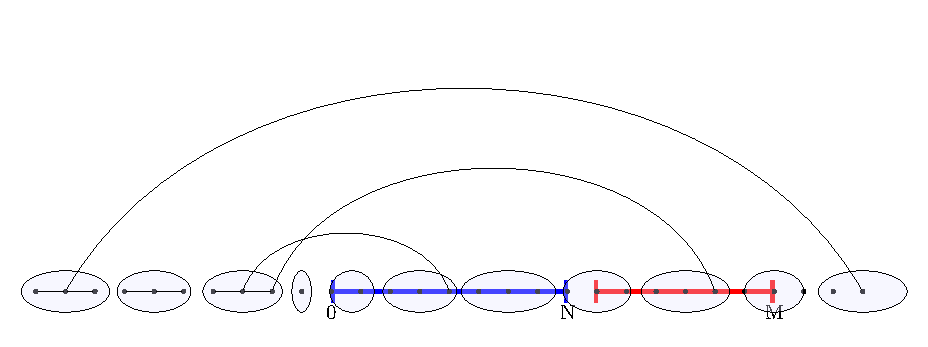
\includegraphics[page=1,width=0.9\textwidth]{fig.pdf}\]

The one-sided Ising model $\nu(x)$ is obtained from the random cluster model with respect
to spins in $V_+$ and the Bernoulli graph model of $\t^+$. 
We may write the marginal of the cylinder $\cy N$ for the \emph{one-sided Ising model} as
\[
  \nu(\cy N) =
  \frac{\XI{ 2^{\ol\omega_S(\t^+)} \cdot b(\t^+,\cy N)}}{\XI{2^{\omega(\t^+)}}}
  = \frac{\XI{ 2^{\ol\omega_S(\t^+) + f(\t')} \cdot b(\t^+,\cy N)}}{\XI{2^{\omega(\t^+)+f(\t')}}}.
\]
where $f(\t')$ denotes an arbitrary function of the graph $\t'$. 

\def\M{{M}}
\def\N{{N}}



Our aim is to show that for all $x\in\SI^{[0,\infty)}$
\[
  \lim_{M,L\to\infty} \frac{\mu(\cy \M \mid \cy \N)}{\nu(\cy\M \mid \cy\N)} = 1+\ordo N \quad\text{as $N\to\infty$.}
\]

We have
\[
\mu([x]_M|[x]_N)\propto \frac{\XI{ 2^{\ol\omega_M(\t)} \cdot b(\cy M,\t)}}{\XI{ 2^{\ol\omega_N(\t)} \cdot b(\cy N,\t)}},
\]
where we have $\ol\omega_M(\t)=\ol\omega_N(\t)-K_{M,N}(\t)$ and 
$b(\cy M),\t)=b(\cy N,\t)\cdot \tilde b_{M,N}(\t)$. Similarly, we have
\[
\nu([x]_M|[x]_N)\propto \frac{\XI{ 2^{\ol\omega_M(\t^+)} \cdot b(\cy M,\t^+)}}{\XI{ 2^{\ol\omega_N(\t^+)} \cdot b(\cy N,\t^+)}},
\]
where $\ol\omega_M(\t^+)=\ol\omega_N(\t^+)-K_{M,N}(\t^+)$ and 
$b(\cy M,\t^+)=b(\cy N,\t^+)\cdot \tilde b_{M,N}(x,\t^+)=\tilde b_{M,N}(x,\t)$. 

We now prove that $\XI{T<N}=1-o(1)$, as $N\to \infty$.

We define a correction term $C_N(\t',\t^+)$ by the identity $$\ol\omega_N(\t)-\ol\omega_N(\t^+)=f(\t')+C_N(\t',\t^+).$$ 

We can prove that this correction term is bounded, which follows from the inequality 
$$
C_N(\t',\t^+)\leq 
E(C_k^2) \cdot \sum _{k=1}^\infty \frac{1}{(N+k)k}<\infty,
$$
where $C_k$ are clusters in $\t[(-\infty, 0])$ ordered after $M(C_k)$,
$M(C_k)\geq k$, and $M(C)=\min \{-i : i\in C \}$.

Conditioned on the event $N>T$, we have that $K_{M,N}(\t^+)=K_{M,N}(\t)$ and that $\tilde b_{M,N}(\t^+)=\tilde b_{M,N}(\t)$.

From the computations above we deduce that 
\[
  \frac{\mu(\cy\N)}{\nu(\cy\N)} = \text{const.} \times
  \frac{\XI{2^{\ol\omega_\N(\t)} \cdot b(\t,\cy\N)}}
  {\XI{2^{\ol\omega_\N(\t^+) + f(\t')} \cdot b(\t^+,\cy\N)}}
\]
where the constant is \({\XI{2^{\omega(\t^+)}}}/{\XI{2^{\omega(\t)}}}\).


Then
\begin{equation}
  \ol\omega_N(\t) = \ol\omega_N(\t^+) + \ol\omega_N(\t^-) - X_N(\t') + Z_N(\t)
\end{equation}
where $X_N(\t')$ are the number of edges between clusters in $\mscr R^-_N$ and
$\ol N$. The term $Z_N(\t)$ is a correction term which is not independent of $\t^+$.
However, we have
\[ Z_N(\t) \le Y_N(\t')\]
where $Y_N(\t)$ is the number
\[
  Y_N(\t') = \sum_{C\in\mscr R^-_N} \max\{|E(C,\ol N)|-1,0\}
\]
We claim that $Y_N(\t')$ has distribution bounded by a Poisson variable
$\opn{Po}(\lambda_N)$ where $\lambda_N\to 0$ as $N\to\infty$. 


We let 
$$A_N^{(m)}= \int 2^{\overline{\omega}([0,N), G^{(m)}}\cdot B([x]_N,G^{(m)}) \; d\xi (G),$$
$$E=\{(i,j): i<0 \wedge j\geq 0\},$$
$$G^{(m)}=G^+ \cup G^- \cup \{(i,j)\in E: |i|+|j|\leq m\},$$
and
$$r^{(m)}=|G^{(m)}\cap E|.$$
We claim that there exist uniform constants $c_1$ and $c_2$ such that
$$0<c_1\frac{A_N^{(m)}}{A_N^{(0)}}<c_2<\infty,$$
where we study $A_N^{(m)}$ such that we have in the extremes
$$A_N^{(0)}=\nu([x]_N)$$
and 
$$A_N^{(\infty)}=K\cdot \mu([x]_N).$$

We have 
$$X^{(m)}=K\cdot \int 2^{\overline{\omega}_n(G^{(m)})-r^{(m)}(G)}\cdot B([x]_m, G^{(m)})\; d\xi(G),$$
so that
$$X^{(0)}=\nu([x]_n)$$
and
$$\lim_{m \to \infty} X^{(m)}=C\cdot \mu([x]_n).$$ 
We have furthermore
$$X^{(0)}\geq X^{(1)}\geq \ldots,$$
but we need to prove that the monotone sequence is bounded away from zero.

We have
$$\nu([x]_n)=\frac{ \int 2^{\omega_n(G^+)}\cdot 2^{-\omega_n(G^+)}\cdot B([x]_n, G^+)\; d\xi(G)}{\int 2^{\omega_n(G)} \; d\xi(G)  },$$
where $G^+=G^{(0)}$, and 
$$\mu([x]_n)=\frac{ \int 2^{\omega_n(G)}\cdot 2^{-\omega_n(G^)}\cdot B([x]_n, G)\; d\xi(G)}{\int 2^{\omega_n(G)} \; d\xi(G)  }.$$



Let 
$$K_m=\min \{|i|: i\in C_m\},$$
where $C_m$ is the $m$th cluster. Note that $K_m\geq m$.

We will prove that if $A_n$ is the event that we send one edge from the negative to the positive side (beyond 0), as well as one edge from the negative side beyond $n$, then $P(A_n)\to 0$.

The probability of an edge from cluster $C_i$ (e.g.\ on the negative side) to cluster $C_j$ (e.g.\ on the positive side) is
$$1-e^{-\sum_{C_i} \frac{\beta}{|i-j|^{\alpha}}}.$$ 

We have
$$\sum_{-k\in C}\frac{\beta}{n+k}\leq |C|\cdot \frac{1}{K_C}\cdot \beta.$$
Hence the probability of valence $\geq 2$ is 
$$\leq  |C|^2\cdot \frac{1}{K_C^2}\cdot \beta^2.$$
Since then
$$\sum \frac{C_m^2}{K_m^2}<\infty,$$
we have by the Borel--Cantelli lemma only finitely many clusters with valence $\geq 2$.





\section{Nytt}
\hrule 

Let $G=(G^+, G^- , E)$, $\gamma=(G^+,G^-)$.

We have
$$d\tl\nu(G)=2^{\omega(G^+)+\omega(G^-)-|E|-\rho_{|E|}}\; d\xi(G),$$
where $\xi$ is the Bernoulli measure, and $E$ is the set of edges from the minus side to the plus side. The term $\rho_{|E|}$ normalises, i.e.\ 
\[
\rho_{|E|} = 
\log \int 2^{\omega(G^+)+\omega(G^-)-|E|}\; d\xi(G).
\]
Notice that
$\omega(G^-)-|E|$ is independent of $G^+$, and so we have $\nu\circ (G^+)^{-1}=\nu(G^+)$.

We have 
$$d\mu(G)=2^{q(G)-\rho_q}\; d\nu(G),$$
where $\rho_q$ just normalises $\mu$ and where $q(G)$ is the co-rank in the set $E$, i.e., 
$$
q(G)=\max \{|E|-|T\cap E|\mid \text{$T$ spanning tree of $G$} \}.
$$
Consider the graph $G_{ij}\subset E$ where for $i,j>0$
$$ G_{ij} =  \gamma \cup 
\{ kl\in E \mid k < i \text{ or } k=i \text{ and } 0>l>-j \}.
$$
We also denote $G_m = \lim_{j\to-\infty} G_{mj}$. 
We can define $q(G)$ as the number of edges between $i$ and $-j<0$ that connects vertices ``already'' connected in $G_{ij}$. 
It is also clear that $q$ is less than or equal to the number of 
cluster in $G^-$ incident with more than one edge of $E$.


We claim that,
$$
P(q|\gamma)\approx \operatorname{Po}(\lambda(\gamma))
$$
where $\lambda(\gamma) = \mathsf E(q|\gamma)$. We have 
\[
\lambda(\gamma) = \sum_{i=0}^{\infty} \sum_{j=1}^{\infty} (1-e^{-\frac{\beta}{(i+j)^2}}) 
\mathsf P(i\sim_{G_{ij}} -j\mid \gamma).
\]
where $a\sim_H b$ states that there is a path between $a$ and $b$ in the graph $H$. 

Since $G_{ij}$ is stochastically dominated by $G$ we obtain that 
\[
\P(i \sim_{G_{ij}} -j) \le \P(i \sim_G j) = \tau(i+j),
\]
where $\tau(n)$ is the usual two-point correlation function 
\[
\tau(n) = \mathsf P(0\sim_G n).  
\]
Hence, 
\[
\mathsf E(\lambda(\gamma)) \le
\sum_{i=0}^\infty 
\sum_{j=1}^\infty \frac\beta{(i+j)^2} \tau(i+j) = 
\beta \sum_{n=1}^\infty \frac {\tau(n)}n
\]

We need to show that $\E(e^{\lambda(\gamma)})<\infty$, since, from
the Poisson approximation it follows that 
$$
g(\gamma)=E(2^{q(G)}|\gamma) \approx e^{\lambda(\gamma)}.
$$
Then we have 
$$\frac{d\mu(\gamma)}{d\nu(\gamma)}=g(\gamma) < \infty. $$


For a fixed sequence $x\in\{-1,+1\}^{\ZZ_+}$, 
let the measure $\nu(\cdot;[x]_n)$ be defined by
\[
\d\nu\ii n(\gamma) = 
\d\nu(\gamma; [x]_n) =
B(\gamma,[x]_n) 2^{\ol\w_n(\gamma)} \d\eta(\gamma).
\]
That is, $\nu(\gamma; [x]_n)$ is $\nu(\gamma)$ conditioned on $\gamma$ 
and $[x]_n$ being compatible. 
Note that $\nu\ii n \prec \nu\ii {n-1}$ in the stochastic dominance order since 
$B(\gamma; [x]_n)$ is a decreasing event. 
Thus $\tau\ii {n+1} (k) \le \tau\ii n (k) \le \tau(n)$. 
We have
\[
\nu([x]_n) = \int \d\nu\ii n(\gamma)
\]

Let $b_n(G)=\frac{B(G,[x]_n)}{B(\gamma,[x]_n)}$. 
We consider 
\begin{gather*}
\log \frac{d\mu([x]_n)}{d\nu([x]_n)}
=
\log {\int \int b_n(\gamma,E)\, 2^{q(\gamma,E)} \, 2^{|E|}\, \d\eta(E)\, d\nu\ii n (\gamma; [x]_n)} \\
-  \log {\int \int 2^{|E|} \d\eta(E)\, d\nu\ii n(\gamma; [x]_n) } + \text{constant}
\end{gather*}
We aim to show that this is bounded, i.e.\ that for all $n$ 
\begin{equation}
  |\log \frac{d\mu([x]_n)}{d\nu([x]_n)}| \le K 
\end{equation}
We claim that this holds with $K$ of the order
\[
K(\beta) = \beta \sum_{n=1}^\infty \frac{\tau(n)}{n}.
\]

\[
=\frac{\int2^q 2^{-\omega_n} B\; d\nu}{\int 2^{-\omega_n^+} B^+\; d\nu }
=\frac{\int b_n \cdot 2^{q-r_n}\cdot 2^{-\omega_n^+}\cdot B^+\; d\nu}{\int 2^{-\omega_n^+} B^+\; d\nu},
\]

Hence by defining 
$$h_n(\gamma)=\int b_n \cdot 2^{q-r_n}\; d\xi(G),$$
we have
$$f_n=\frac{\int h_n(\gamma)2^{\omega_n^+}\cdot B^+\; d\nu}{\int 2^{\omega_n^+} B^+\; d\nu},$$
and we can obtain an upper bound of $f_n$ by bounding $g(\gamma)$.

\subsection{Continuity??}
Let $k$ be a fixed positive integer, and consider
$$h_{n+k}=\int \frac{b_{n+k}\cdot 2^{-r_{n+k}}}{b_n \cdot 2^{r_n}}\cdot 2^{r_n}\cdot b_n\; d\xi(E).$$
In order to prove we want to prove that $\lim_{n\to \infty} \frac{b_{n+k}}{b_n}=1$ in probability, as well as 
$\lim_{n\to \infty} \frac{b_{n+k}2^{-r_{n+k}}}{b_n 2^{r_n}}=1$ in probability.

We can write 
$$h_n{\gamma}=\int b_n r^{-r_n}\cdot 2^q \; d\xi(G|\gamma),$$
which we claim is decreasing monotonically to 
$$\int b_n r^{-r_\infty}\cdot 2^q \; d\xi(G|\gamma).$$


\section{New April 21}

We think we also can have a finite 
$$\frac{d\mu(\gamma)}{d\nu(\gamma)}= 2^{r(\gamma)}-c$$
where $r(\gamma)\leq \beta \sum \frac{\tau (n)}{n}$.

Let $X$ be the number of components in $\gamma_{-}$, where $d(E,\gamma)\geq 2$. Then we have (something like)
$$E(X)\leq \beta^2 \sum_{k=1}^\infty\left(\sum_{j=k}^\infty \frac{\tau(j)}{j}\right)^2\cdot K.$$

We define $\rho_j$ as the probability of having a path from 
$-j$ to some vertex in $[0,\infty)$. The number of corrections we need to do gives a contribution 
$$\frac{\beta}{(i+j)^2}\cdot \rho_j,$$
where we have $\rho_j^{i}\leq \frac{\beta}{(i+j)^2} \cdot \rho_j$. We get a sum 
$$\sum_{i=1}^\infty \sum_{j=1}^\infty \frac{\beta \rho_j}{(i+j)^2}.$$ 

Let $C(0)$ be the cluster that contains $0$. We have for a uniformly chosen cluster $C$ that $|C_+(0)|<|C|$.

We can now study
$$\frac{dP(|C(0)|)}{dP(|C|)}$$
where
$$\frac{P(|C(0)|=x)}{P(|C|=x)}=\frac{x}{E(|C|)}.$$

We let $X$ be the number of components in $\gamma_{-}$ so that $d(E,\gamma)\geq 2$ and $Y=|C_+(0)|$. 

A crude estimate gives
 $$ 
 \E(X)\leq \sum_{k=1}^\infty E \left( \frac{Y_k}{k}\right)^2<\infty.  
 $$ 
 We obtain 
 $$\frac{1}{E(|C|)}\cdot E Y^2\leq E \left(\frac{|C|^2}{E(|C|)}\right)=E(C(0))<\infty.$$
 
 (We have stochastic dominance order as we move to the left, e.g.,  $Y_2 \prec Y_1$.
 
 We will from these considerations derive uniform convergence of $h_n$ to $h$, which then needs to be a continuous function (Cauchy's theorem):
 $$ \|h_n(x)-h_m(x)\|_{\infty}\leq K\cdot \sum_{k=n}^\infty \frac{\rho_k}{k}.$$
 
 We consider $\omega(G)=\omega (\gamma)-|\epsilon|+ R(\gamma, \epsilon)$, where $G=\gamma \cup \epsilon$, and we have 
 $$\nu(\gamma,\epsilon) \propto 2^{\omega(\gamma)-|\epsilon|}$$
 $$\mu(\gamma,\epsilon)\propto 2^{\omega (G)}= 2^{\omega(\gamma)-|\epsilon |+R(\gamma,\epsilon)}.$$
 We define on all of $G$:
 $$\frac{d\mu(G)}{d\nu(G)}=2^{R(\gamma,\epsilon)-c}.$$
 We have
 $$E \left[2^{R(\gamma, \epsilon)}\right] =
 \Ordo{2^{\beta \sum_{n=1}^\infty \frac{\tau(n)}{n}}}.$$
 
 In order to avoid bad paths that do not give rise to cycles, we consider now $B_n(x,\gamma)\searrow B_\infty (x,\gamma)$.
 
 We have $E(B_\infty (x))>c>0$ and 
 $$B_ n(x,G)=C_n(x, \gamma, \epsilon )\cdot B_n(x,\gamma),$$
 where $C_n(x,\gamma, \epsilon)\searrow C_\infty (x,\gamma, \epsilon)$.
 
 We can write
 $$h_n(x)=\int C_n(x,\gamma,\epsilon) \cdot 2^{Q_n(\gamma,\epsilon) }\; d\eta(\epsilon)\cdot 2^{-|\epsilon|} d\alpha.$$
 That is, 
 $$h_n-h_m=\int C_n(x,\gamma,^{(n)},\epsilon)2^{Q(\gamma^{(n)},\epsilon)}-C_m(x, \gamma^{(m)},\epsilon)2^{Q(\gamma^{(m)},\epsilon)}d\eta(\epsilon)\cdot 2^{-|\epsilon|} d\alpha(\gamma^{(n)},\gamma^{(m)}).$$
 
 We have $\gamma^{(m)}\subseteq \gamma^{(n)}$ and 
 $$\int |Q_m(\gamma,\e)-Q_n(\gamma,\e)|\; d\mu(\gamma,\epsilon)\leq K\cdot \sum_{j=m}^n \frac{\rho_j}{j}.$$
 Since we also have $0\leq C_m \leq 1$ and 
 $$c_m(\gamma,x)\cdot 2^{q_m(\gamma)}=\int C_m(x,\gamma,\epsilon)2^{Q_m (\gamma,\epsilon)-|\epsilon|}\; 2^{-|\epsilon|} \, d\eta(\epsilon),$$
 we obtain
 $$h_n-h_m=\int c_n(\gamma,x)2^{q_n(\gamma^{(n)})}-c_m(\gamma,x)2^{q_m(\gamma^{(m)})} \; d\alpha(\gamma)$$
 $$=\int \left(c_n(\gamma^{(n)})-c_m(\gamma^{(m)}) \right)2^{q_n(\gamma^{(n)})}\; d\alpha
 +\int c_m(\gamma^{(m)})\left(2^{q_n(\gamma^{(n)})}-2^{q_m(\gamma^{(m)})} \right) \; d\alpha.$$

 Observe that $C_n$ is zero if $B_n(x,G)=0$ and $B_n(x,\gamma)=1$; otherwise $C_n$ is equal to $1$.

 The following lemma concludes our proof.
 \begin{lemma}\label{bounds}
   For
   \[ S_n = \beta \sum_{k=n}^\infty \frac{\rho_k}{k} \]
   We have that following
   \begin{align}
     \label{cnbound}
     \int \left(c_n(\gamma^{(n)})-c_m(\gamma^{(m)}) \right)2^{q_n(\gamma^{(n)})}\; d\alpha
     &= \Ordo{S_n - S_m}\\
     \label{qnbound}
     \int c_m(\gamma^{(m)})\left(2^{q_n(\gamma^{(n)})}-2^{q_m(\gamma^{(m)})} \right) \; d\alpha
     &= \Ordo{S_n-S_m}
   \end{align}
 \end{lemma}

 \begin{proof}[Proof of Lemma~\ref{bounds}]


 \end{proof}
 

 


\begin{thebibliography}{999}

\bibitem{ACCN} M.\ Aizenman, J.\ Chayes, L.\ Chayes and C.\ Newman,
  Discontinuity of the magnetization in the one-dimensional
  $1/|x-y|^2$ Ising and Potts models, {\em J.\ Statist.\ Phys.\ } {\bf
    50} (1988), 1--40.

\bibitem{berger} N.\ Berger, C.\ Hoffman and V.\ Sidoravicius,
  Nonuniqueness for specifications in $\ell^{2+\epsilon}$, to appear (2017)
  in {\em Ergodic Theory Dynam.\ Systems}.

\bibitem{berbee87} H. Berbee, Chains with Infinite Connections:
  Uniqueness and Markov Representation, {\em Probab.\ Theory Related
    Fields} {\bf 76} (1987), 243--253.
 
\bibitem{berbee89} H. Berbee, Uniqueness of Gibbs measures and
  absorption probabilities, {\em Ann.\ Probab.\ } {\bf 17} (1989),
  no.\ 4, 1416--1431.
 
\bibitem{lop1} L.\ Cioletti and A.\ Lopes, Interactions,
  Specifications, DLR probabilities and the Ruelle Operator in the
  One-Dimensional Lattice, preprint, arXiv:1404.3232.
 
\bibitem{lop3} L.\ Cioletti and A.\ Lopes, Ruelle Operator for
  Continuous Potentials and DLR-Gibbs Measures, preprint,
  arXiv:1608.03881v1.
 
\bibitem{FS} J.\ Fr\"olich and T.\ Spencer, The phase transition in
  the one-dimensional Ising Model with $1/r^2$ interaction energy,
  {\em Comm.\ Math.\ Phys.\ } {\bf 4} (1982), no.\ 1, 87--101.

\bibitem{johob} A.\ Johansson and A.\ \"Oberg, Square summability of
  variations of $g$-functions and uniqueness of $g$-measures, {\em
    Math.\ Res.\ Lett.\ } {\bf 10} (2003), no.\ 5--6, 587--601.
    
\bibitem{jop1} A.\ Johansson, A.\ \"Oberg and M.\ Pollicott, Countable
  state shifts and uniqueness of $g$-measures, {\em Amer.\ J.\ Math.\
  } {\bf 129} (2007), 1501--1511.  


\bibitem{jop2} A.\ Johansson, A.\ \"Oberg and M.\ Pollicott, Unique
  Bernoulli $g$-measures, {\em J.\ Eur.\ Math.\ Soc.\ } {\bf 14}
  (2012), 1599--1615.
  
\bibitem{keane} M.\ Keane, Strongly mixing $g$-measures, {\em Invent.\
    Math.\ } {\bf 16} (1972), 309--324.

\bibitem{sin}
Ya.G.\ Sinai, Gibbs measures in ergodic theory, {\em Russian Mathematical Surveys} {\bf 27}(4) (1972), 21--69. 

\bibitem{walters1}
P.\ Walters, Ruelle's operator theorem and $g$-measures, {\em Trans.\ Amer.\ Math.\ Soc.\ } {\bf 214} (1975), 375--387.

\bibitem{walters3}
P.\ Walters, Convergence of the Ruelle Operator, {\em Trans.\ Amer.\ Math.\ Soc.\ } {\bf 353} (2000), 
no.\ 1, 327--347.
\end{thebibliography}

\noindent
\newline

\noindent
Anders Johansson, Department of Mathematics, University of G\"avle,
801 76 G\"avle, Sweden. Email-address: ajj@hig.se\newline

\noindent
Anders \"Oberg, Department of Mathematics, Uppsala University, P.O.\
Box 480, 751 06 Uppsala, Sweden. E-mail-address:
anders@math.uu.se\newline

\noindent
Mark Pollicott, Mathematics Institute, University of Warwick,
Coventry, CV4 7AL, UK. Email-address: mpollic@maths.warwick.ac.uk\newline

\noindent
Evgeny Verbitskiy, Mathematical Institute, Leiden University,
Niels Bohrweg 1, 2333 CA Leiden, The Netherlands. E-mail address: evgeny@math.leidenuniv.nl




\end{document}
